Se encarga al inicio de la aplicación, de acceder a la tarjeta uSD para obtener la lista de canciones y la configuración guardada. Cuando se le indica, se encarga de guardar la configuración actual para poder iniciarse en el próximo encendido con la misma configuración. 

Para su desarrollo, primero intentamos utilizar el driver \texttt{SD} de la placa \texttt{STM32F769I-Disco}, la librería \textit{FatFs} \cite{FatFsModuleApplication}\cite{FatFsGenericFAT} y una tarjeta micro-SD.

Hemos decidido almacenar en la tarjeta el siguiente contenido:
- \texttt{songs.txt}: Lista de canciones. Máximo puede haber 25 canciones, de 30 caracteres cada una (29 en Windows debido al salto de línea). 
- \texttt{config.txt}: Configuración del sistema. Valor de las 5 bandas de ecualización y del volumen.


La estructura del código necesario para este proyecto es:
- FatFs:
	- \texttt{ff.c}, \texttt{ff.h}
	- \texttt{ff_gen_drv.c}, \texttt{ff_gen_drv.h}
	- \texttt{diskio.c}, \texttt{diskio.h}
	- \texttt{sd_diskio.c}, \texttt{sd_diskio.h}
- uSD:
	- \texttt{sd.c}, \texttt{sd.h}
	- \texttt{fatfs_storage.c}, \texttt{fatfs_storage.h}

FatFS es un módulo genérico de sistena de archivos FAT/exFAT para pequeños sistemas embebidos. Es independiente de la plataforma en la que se utilice. Está compuesto por las librerías mencionadas en la estructura.

FatFs se utiliza como abstracción sobre el sistema de ficheros Fat. En nuestro nivel de aplicación solo necesitamos llamar a las funciones de fichero \texttt{ff}. Sin embargo, tenemos que crear una clase que permita unir las librerias FatFs (mediante \texttt{diskio.h}) con la implementación hardware de la uSD. Nosotros utilizamos para ello la clase \texttt{sd_diskio}, mediante el Board Support Package (BSP) de la \texttt{STM32F769I-Disco}.

\begin{figure}[h]
    \centering
    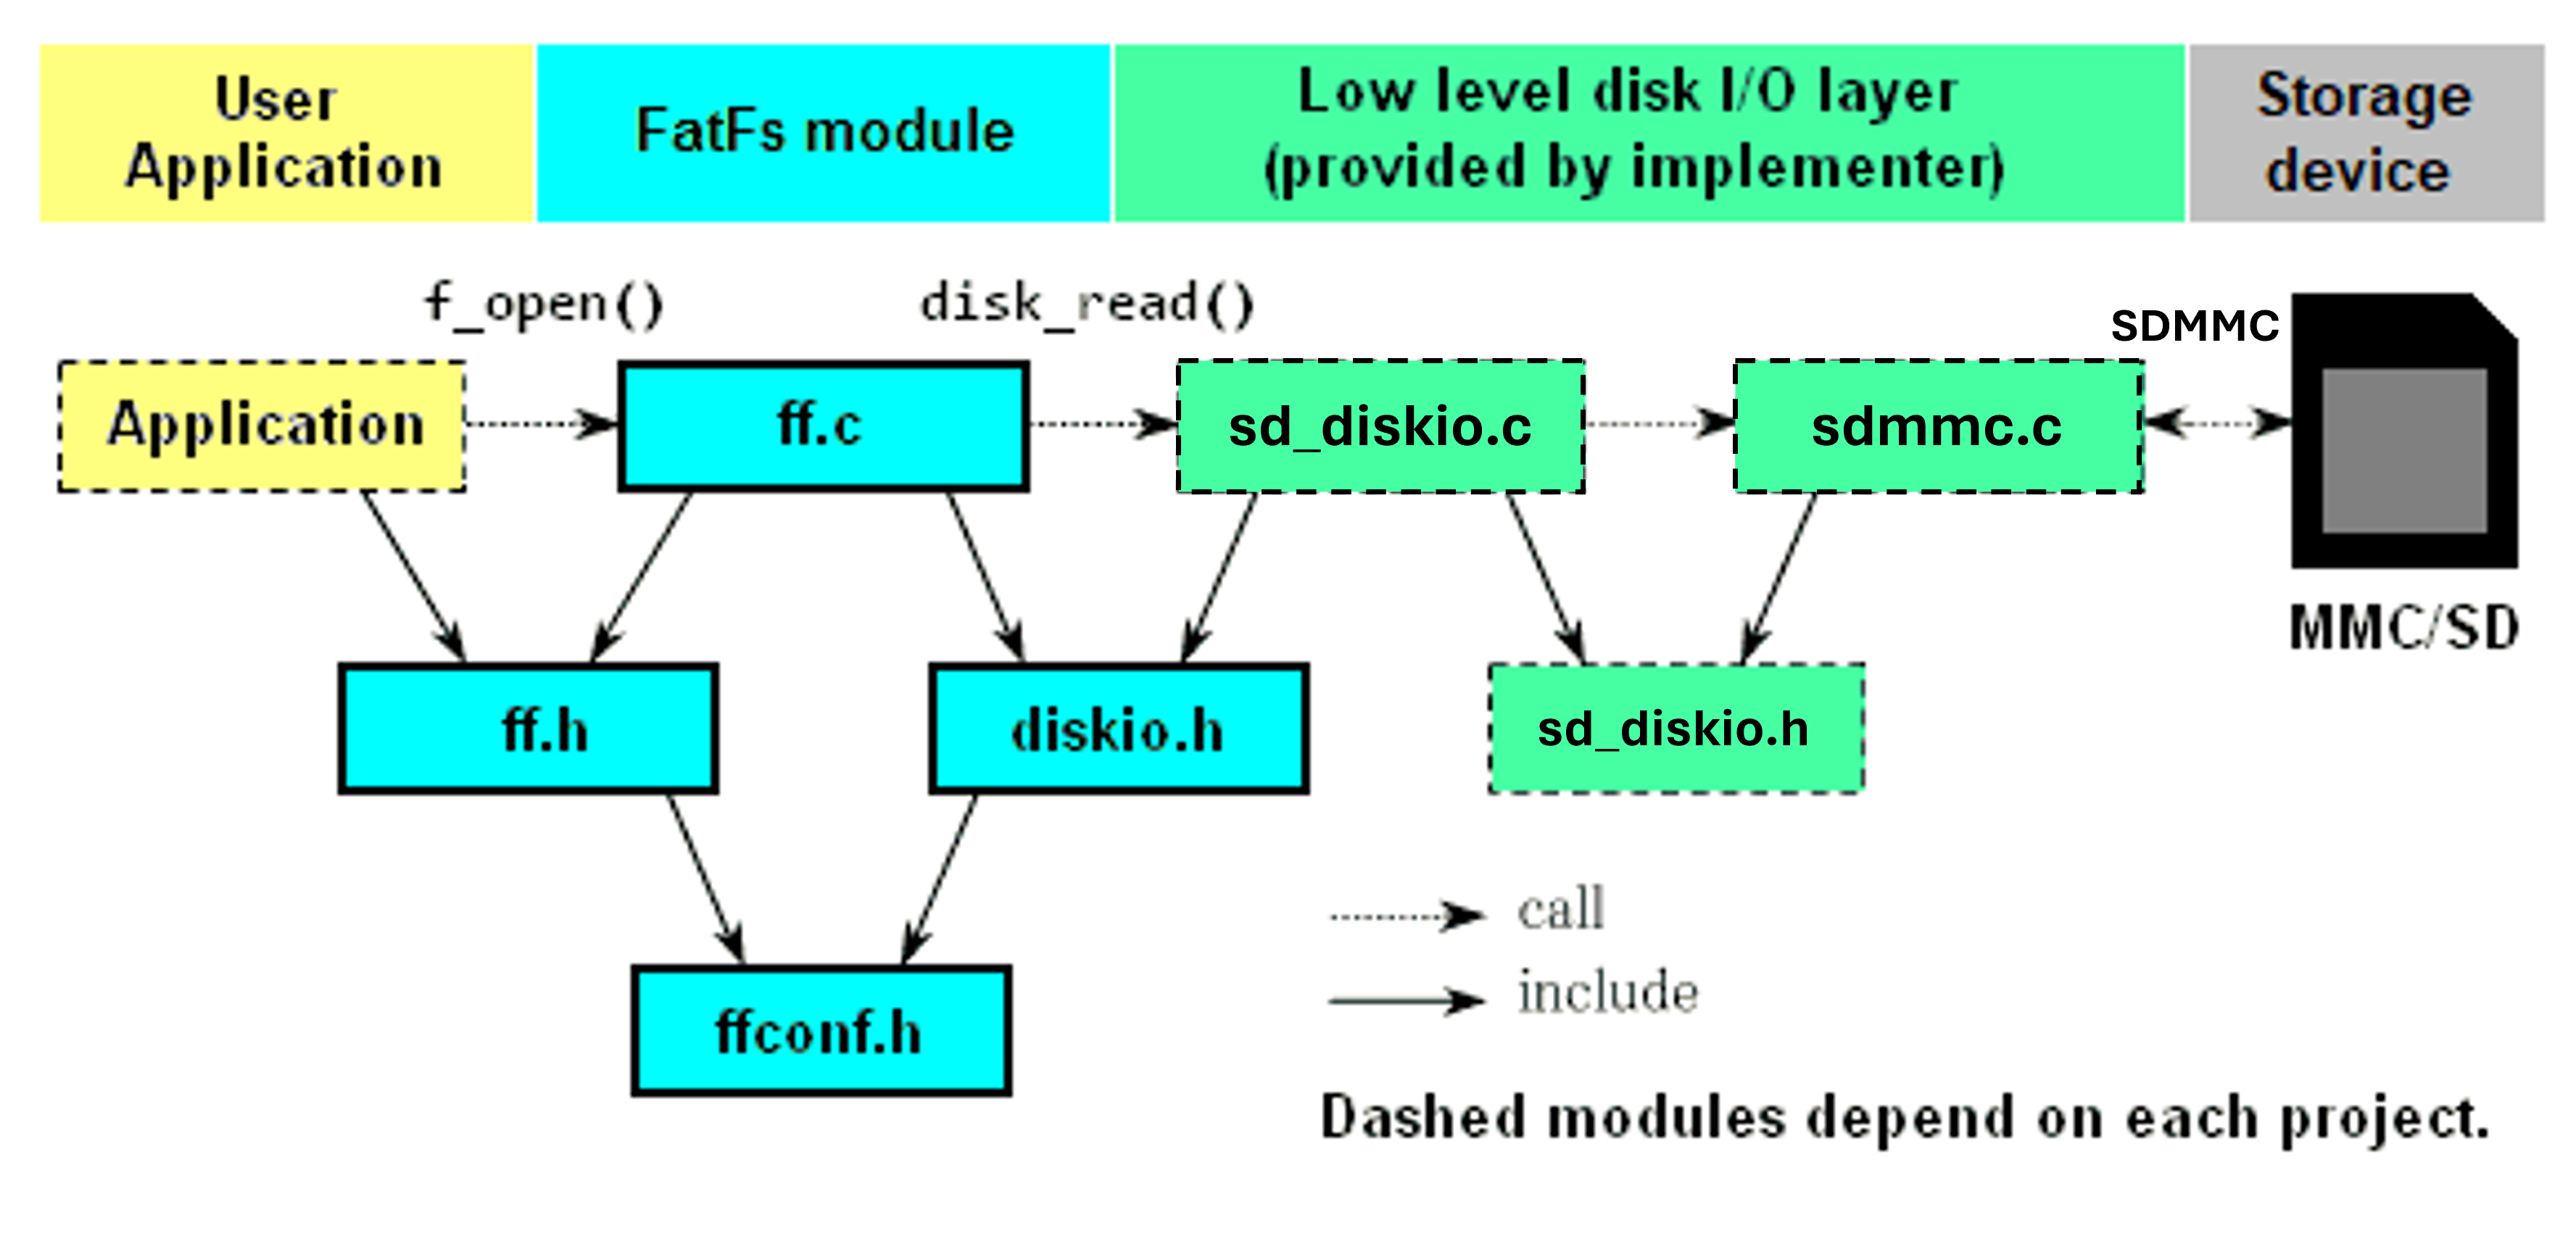
\includegraphics[width=0.5\textwidth]{images/3/3-2/SD/FatFs_1.png}
    \caption{Configuración del sistema implementando FatFs}
    \label{fig:sistema-fatfs}
\end{figure}

Los ficheros \texttt{sd.c} y \texttt{sd.h} se encargan de inicializar la tarjeta, obtener la lista de canciones y la configuración guardada, y de guardar la configuración actual. Esto lo hace utilizando las funciones definidas en \texttt{fatfs_storage.h}. Además, se encarga de revisar que los valores son correctos y están en el rango adecuado. Si no están dentro del rango, los modifica al valor más cercano dentro del rango. También se encarga de adaptar todo lo obtenido a los tipos de variables correctos para la integración del proyecto.

En primer lugar, se inicializa la uSD con la función pública \texttt{Init_SD}. Basicamente se monta la tarjeta y se obtienen el directorio, las canciones (\texttt{Get_Songs}) y la configuración guardada (\texttt{Get_Config}). Toda la información se guarda en punteros a variables del control. Después, cuando se quiere guardar la configuración, se llama a la función pública \texttt{Save_Config}.

Para parsear toda la información lo hacemos de la siguiente manera:

\begin{itemize}
	\item Parseo de la lectura de la configuración: Utilizamos un \texttt{sscanf}.
	\item Parseo de la lectura de las canciones: Utilizamos un algoritmo de copia de cadena de caracteres de triple puntero.
	\item Parseo de la escritura de la configuración: Utilizamos un \texttt{sprintf}.
\end{itemize}

\texttt{fatfs_storage.c} y \texttt{fatfs_storage.h} se encargan de las operaciones de lectura y escritura de los archivos. Esto lo lleva a cabo mediante llamadas a las funciones de las librerías de FatFs. Tiene tres funciones diferentes:

\begin{itemize}
    \item Storage_GetDirectoryBitmapFiles: Se monta la tarjeta con f_mount y se obtiene el directorio de ficheros. El directorio se obtiene llamando a la función de FatFs \texttt{find_first} y después con \texttt{find_next} mientras existan más ficheros. Al final, se cierra el directorio con \texttt{closedir}. (\texttt{f_mount} -> \texttt{f_findfirst} -> \texttt{f_findnext} -> \texttt{f_closedir}).
    \item Storage_OpenReadFile: Se lee un archivo. Primero se abre el archivo, después se lee y finalmente se cierra. (\texttt{f_open} -> \texttt{f_read} -> \texttt{f_close}).
    \item Storage_OpenWriteFile: Se escribe en un archivo. Primero se abre el archivo, después se desplaza el puntero de escritura al principio del fichero .txt y se escribe en él. Finalmente se cierra. (\texttt{f_open} -> \texttt{f_lseek} -> \texttt{f_write} -> \texttt{f_close}).
\end{itemize}

Sin embargo, a la hora de realizar la integración con el resto del proyecto, no funcionaba. La tarjeta llegaba a montarse de manera correcta, pero a la hora de buscar los ficheros, devolvía un \texttt{RXOVER}, que indica que la transferencia de lectura ha sufrido de overflow. 


